\documentclass[onecolumn, draftclsnofoot,10pt, compsoc]{IEEEtran}
\usepackage{graphicx}
\usepackage{url}
\usepackage{setspace}

\usepackage{geometry}
\geometry{textheight=9.5in, textwidth=7in}

\usepackage{graphicx}
\graphicspath{{images/}}

% 1. Fill in these details
\def \CapstoneTeamName{		Team Wombat}
\def \CapstoneTeamNumber{		15}
\def \GroupMemberOne{			Victor Li}
\def \GroupMemberTwo{			Ryan Crane}
\def \GroupMemberThree{			Nicholas Wong}
\def \CapstoneProjectName{		Axolotl}
\def \CapstoneSponsorCompany{	}
\def \CapstoneSponsorPerson{		Kevin McGrath}

% 2. Uncomment the appropriate line below so that the document type works
\def \DocType{		%Problem Statement
				Requirements Document
				%Technology Review
				%Design Document
				%Progress Report
				}
			
\newcommand{\NameSigPair}[1]{\par
\makebox[2.75in][r]{#1} \hfil 	\makebox[3.25in]{\makebox[2.25in]{\hrulefill} \hfill		\makebox[.75in]{\hrulefill}}
\par\vspace{-12pt} \textit{\tiny\noindent
\makebox[2.75in]{} \hfil		\makebox[3.25in]{\makebox[2.25in][r]{Signature} \hfill	\makebox[.75in][r]{Date}}}}
% 3. If the document is not to be signed, uncomment the RENEWcommand below
%\renewcommand{\NameSigPair}[1]{#1}

%%%%%%%%%%%%%%%%%%%%%%%%%%%%%%%%%%%%%%%
\begin{document}
\begin{titlepage}
    \pagenumbering{gobble}
    \begin{singlespace}
    	
\includegraphics[height=4cm]{coe_v_spot1}
        \hfill 
        % 4. If you have a logo, use this includegraphics command to put it on the coversheet.
        %\includegraphics[height=4cm]{CompanyLogo}   
        \par\vspace{.2in}
        \centering
        \scshape{
            \huge CS Capstone \DocType \par
            {\large\today}\par
            \vspace{.5in}
            \textbf{\Huge\CapstoneProjectName}\par
            \vfill
            {\large Prepared for}\par
            \Huge \CapstoneSponsorCompany\par
            \vspace{5pt}
            {\Large\NameSigPair{\CapstoneSponsorPerson}\par}
            {\large Prepared by }\par
            Group\CapstoneTeamNumber\par
            % 5. comment out the line below this one if you do not wish to name your team
            \CapstoneTeamName\par 
            \vspace{5pt}
            {\Large
                \NameSigPair{\GroupMemberOne}\par
                \NameSigPair{\GroupMemberTwo}\par
                \NameSigPair{\GroupMemberThree}\par
            }
            \vspace{20pt}
        }
        \begin{abstract}
        %6. Fill in your abstract    
		   This document is a SRS or software requirements specification that will outline the purpose, scope, and requirements of the NVIDIA Jetson TX2 infotainment and black box system we are to build. It will discuss the system's constraints, list the assumptions we will make in approaching the development of this system, as well as detail our vision as to how users may interact with the system. Additionally, the document will describe the functionality this system will provide and offer a tentative timetable for the fulfillment of project goals and requirements.
      	\end{abstract}     
    \end{singlespace}
\end{titlepage}
\newpage
\pagenumbering{arabic}
\tableofcontents
% 7. uncomment this (if applicable). Consider adding a page break.
%\listoffigures
%\listoftables
\clearpage

% 8. now you write!
\section{Introduction}
\subsection{Purpose}
The purpose of this software requirements specification (SRS) document is to outline and detail the capabilities of the NVIDIA Jetson TX2 infotainment and black box our group will develop, known henceforth as the Axolotl Infotainment System and Axolotl Software. Doing so will enable us to describe the requirements of the Axolotl Infotainment System and Axolotl Software so that we will all have a detailed understanding of the form factor and capabilities of the deliverable system we will develop. The intended audience for this SRS includes our client, the CS Capstone Instructors, and our group.\par

\subsection{Scope}
Our project entails the development of an infotainment system and black box that can be divided into two products: the Axolotl and the Axolotl Software. The Axolotl will connect vehicle sensors, controllers, receivers, and a touchscreen to a NVIDIA Jetson TX2 computer in a package that can be installed in a vehicle. The Axolotl Software runs on the Axolotl and provides users with media playback, navigation, and vehicle data logging capabilities.\par

\section{Definitions}
\begin{itemize}
	\item NVIDIA Jetson TX2: A versatile, efficient, and high-performance computer made by NVIDIA to be used in robots, drones, and smart cameras.

	\item OBDII: On-Board Diagnostics II, a standardized connector installed in all automobiles sold in the United States since January 1st, 1996. Devices connected via a car's OBDII port can read the vehicle's sensor data on the fly.
	
	\item CAN-bus: Controller Area Network Bus, a system that allows sensors and microcontrollers within a motor vehicle to communicate with each other without a central computer.

	\item LIDAR: Light Detection and Ranging, a method of using laser pulses to determine the 3D properties of a faraway object.

	\item AHRS: Attitude, Heading, and Reference System, a system used in modern aircraft to determine and display roll, pitch, and yaw.

	\item Infotainment: A portmanteau of "��information" and "��entertainment"��. When we use the term "infotainment", we are referring to the center console touchscreen that gives drivers access to information and media in modern cars.

	\item RDS: Radio Data System, a method of transmitting the current track information of an FM radio broadcast.

	\item UPS: Uninterruptible Power Supply, an auxiliary power source that enables a device to function for a limited time if its main power source is unavailable.
	
	\item SATA: Serial Advanced Technology Attachment, an interface standard that connects computers to mass storage devices.
	
	\item MP3: A common digital audio coding format that uses lossy compression. MP3 files are given the .mp3 file extension.
\end{itemize}

\subsection{References}
This SRS references one document, titled "Federal Motor Vehicle Safety Standards; Rear Visibility; Final Rule", Report Number 66 of Volume 79 of the Federal Register, dated April 7th, 2014. This document can be obtained from the US Government Publishing Office at www.gpo.gov.

\subsection{Overview}
The remainder of this SRS contains an overall description of the system we are to develop in terms of the necessary hardware and software. The SRS will describe the intended functionality of the product, how it interfaces with users, and the necessary components that will make the specified functionality and interaction possible. Both requirements and optional features are listed in order of priority and desirability, respectively.

\section{Overall Description}
\subsection{Product Perspective}
The Axolotl Infotainment System is comprised of the Axolotl Head Unit and the Axolotl Software.
The Axolotl Head Unit consists of all of the necessary sensors, receivers, and controller hardware connected physically and wirelessly with the NVIDIA Jetson TX2 system. The Axolotl is designed to be integrated into a car to either provide or replace an in-car infotainment system. Users will not interact directly with the sensors, receivers, or controllers.\par

The Axolotl Software will be installed on the Axolotl Head Unit's TX2 unit and directly interface with the user. The software will operate on Linux, as it is the base operating system installed on the TX2. The Axolotl Software will interact with the hardware and provide users with the ability to control media playback, conduct mapping and routing with navigation, and also exert limited control over system settings.\par

\subsection{Product Functions}
The main functions of the Axolotl are:
\begin{itemize}
	\item	The Axolotl will allow users to play media from multiple sources including: External/Internal storage, Bluetooth, Auxiliary, and FM.
	\item	It will also offer navigation with destination entry, mapping, and offline capabilities. 
	\item	The black box portion of the Axolotl logs output from a dashcam and select sensors tied into a car's OBDII port. Users are able to download the black box data to a storage device or clear all black box data. 
	\item	The Axolotl display will also switch to the backup camera when the car is in reverse.
	
\end{itemize}
\subsection{User Interfaces}
The Axolotl Software will be interacted with via a touch-based graphical user interface divided into the content window and the dock. The dock offers touch zones that will change the content window to either the media, navigation, or system menu. Each content window will have a submenu that displays contextual options and a content box encapsulating the main interactive content that changes based on the option selected in the submenu.\par
\subsection{Hardware Interfaces}
The hardware components of the system will include: an OBDII connector which will receive information from multiple onboard car sensors, an FM receiver for FM radio capabilities, an auxiliary 3.5mm headphone jack adapter, a storage medium for the logging of all sensor data from the car, and a ten-inch HDMI touchscreen that will connect to the TX2 via HDMI.\par
\subsection{User Characteristics}
The Axolotl will be used by ourselves, our client, and the general public: specifically car owners with any level of technological experience.\par
\subsection{Constraints}
\begin{itemize}
	\item We are limited to using the NVIDIA Jetson TX2 as the computing hardware.
	\item The backup camera feed must linger on the screen for 4-8 seconds after shifting out of reverse, in accordance with federal motor vehicle safety standards.
\end{itemize}
\subsection{Assumptions}
\begin{itemize}
	\item This SRS assumes the availability of an accessible WiFi network with internet connectivity.
	\item This SRS assumes the availability of Linux.
	\item This SRS assumes that the hardware used in the Axolotl Head Unit may be changed as necessary to fulfill the listed software requirements; thus, the Axolotl Head Unit will not have rigid specifications other than the required hardware that is specified as a constraint in Section 3.6 of this SRS.

\end{itemize}
\section{Specific Requirements}

\subsection{External Interfaces}
\begin{itemize}
	\item The Axolotl Software is a Linux program that is installed on the NVIDIA Jetson TX2.
	\item Users interact with the Axolotl Infotainment System via a graphic user interface displayed on a touchscreen.
	\item Users are able to control media, navigation, and data settings at any time.

	\begin{itemize}
		\item In the media menu:
	\begin{itemize}
\item Users may select either FM, Aux, USB, Internal Storage, or Bluetooth as the audio source. Users will also be able to turn the audio system off.
	\item Users may change the current FM radio station.
	\item Users may pause/play as well as select previous track/next track while playing media from internal and external storage.
	\item Users may use a volume slider to adjust master audio output volume.
\end{itemize}

		\item In the navigation menu:
\begin{itemize}
\item Users may view the map or input an address and navigate to the destination.
\begin{itemize}
	\item Users may enter the address as house number, street, city, state, and zip code.
\end{itemize}
		\item Users may stop navigation and cancel their route at any time.
	\end{itemize}
		
		\item In the data menu:
		\begin{itemize}
	\item Users may use a toggle switch to turn off the system's WiFi connectivity.
	\item Users may wipe the data stored in the black box. This is only available after entering a password.
\end{itemize}
\end{itemize}

	\item Users will also be able to interact with the system in a minimum of two of any of the following ways:
	\begin{itemize}
 		\item Navigation: Users may choose between 2D flat and 2D topographical maps.
		\item Media: Users can wirelessly download media from a home computer to internal storage.
		\item Data: Users may view a list of OBDII error codes thrown by their vehicle and meaning of these codes.
		\item Data: Users may view their fuel economy statistics and also get tips on how to improve their fuel efficiency.
		\item Media: Users may change the volume and tune radio stations using physical knobs.
		\item Miscellaneous: Users may use a connected Bluetooth device to receive phone calls.
		\item Data: Users may view their AHRS data as it is recorded.
	\end{itemize}

	\item The system receives input from sensors and stores it in a log.
\end{itemize}

\subsection{Functions}
\begin{itemize}
	\item The system will boot using power from a UPS before switching over to vehicle power.
	\item The system will parse incoming RDS data from the current FM radio station to generate FM station information displayed to the user.
	\item The system will search Internal/External storage drives and display a list of playable tracks to the user ordered by filename for playback selection. Playback of .mp3 is supported at minimum.
	\item The black box data log must be saved to a removable storage medium.
	\item The system will automatically play the next song when playing media from internal/external storage.
	\item The system will format data from an OBDII port, connected cameras, and AHRS sensors for logging.
	\item The system will utilize a single GPS receiver unit to determine the vehicle's current location for routing.
	\item The system will compensate for the loss of mobile data signal and allow for offline routing and mapping.
	\item The navigation system will be limited to addresses within the United States.
	\item The system will automatically switch to the backup camera feed when the vehicle is reversing. 
	\item The system will switch off the display when the car turns off, and the Jetson TX2 will enter a standby mode.
	\item The system will also offer a minimum of one of any of the following optional functions:
        	\begin{itemize}
        	\item The system will exert control over microcontrollers to manage supplemental turn signals and backup lights.
        	\item The system will use multiple GPS receivers throughout the vehicle to improve GPS location accuracy.
			\item The system will use a dead reckoning system to compensate for loss of GPS signal.
			\item The system will record dashcam data from both front and back cameras.
        	\item The system will utilize a connected LIDAR system to provide passive parallel parking assist.
	\item The system will utilize the dashcam to detect lane lines and provide lane departure warning.
	\end{itemize}
\end{itemize}

\newpage
\section{Appendix}
\subsection{Project Gantt Chart}
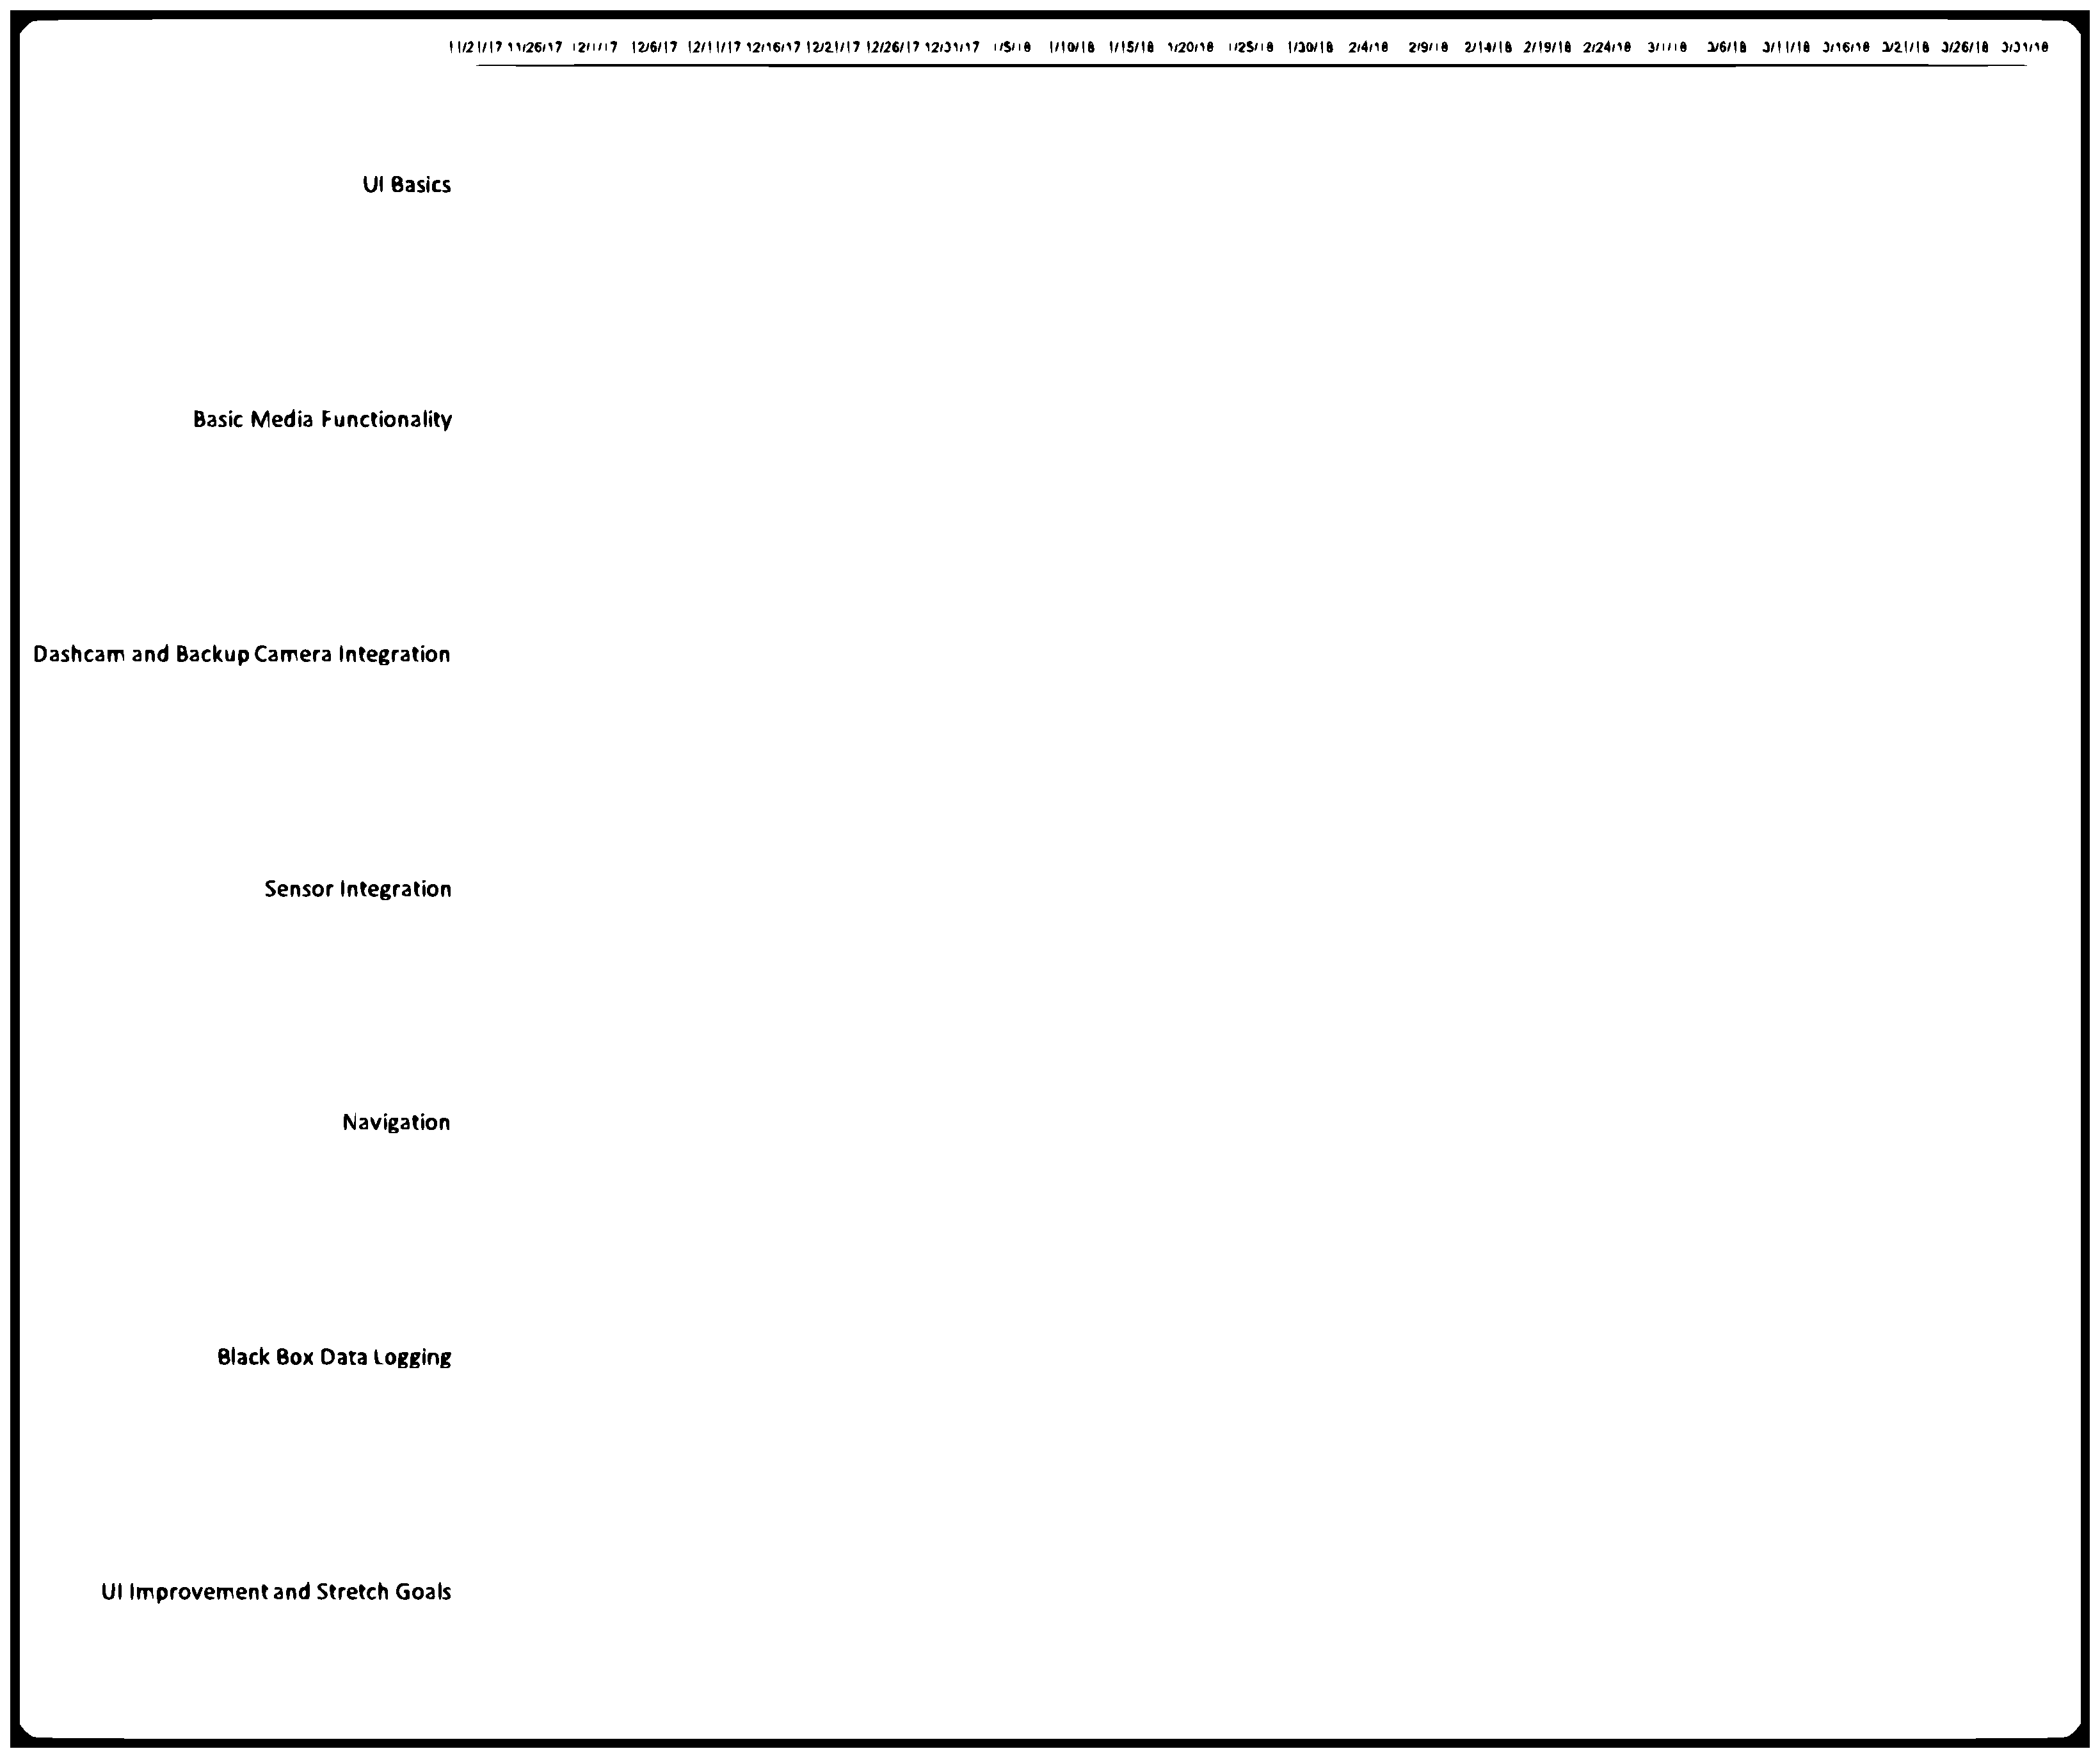
\includegraphics[width=\textwidth ]{gantt.eps}
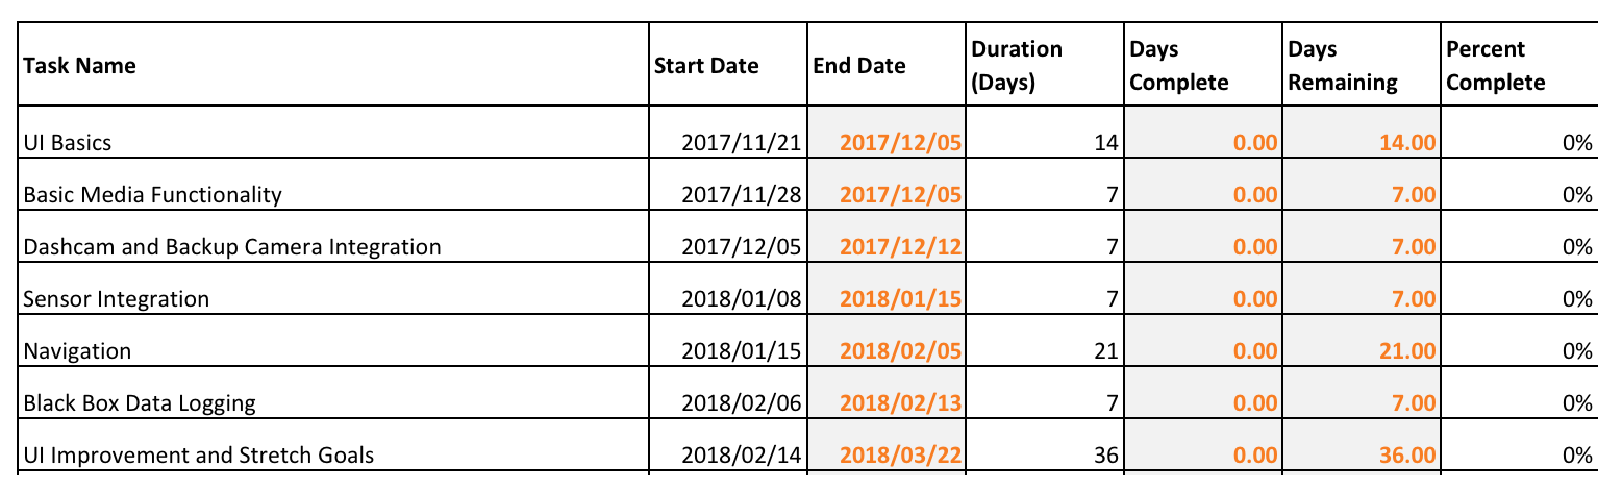
\includegraphics[width=\textwidth]{tablegantt.eps}

\subsection{Change History}
\textbf{December 1st, 2017:} Removed clause stating that users will be able to download data log to removable storage medium. Added clause to functional requirements section stating that data log will be saved to a removable storage medium by default.
\end{document}


